\section{Introduction}

In spite of a host of efforts to diversify the field, computer
science remains a field dominated by white and Asian males.  A
recent Taulbee survey suggests that only 17.9\%
of bachelor's degrees in computer science are awarded to students
identified as female, 3.1\% to students identified as Black or
African-American, and 7.5\% to students identified as Hispanic
\cite{Taulbee2016}.  Many factors likely lead to this
problem.  Unfortunately, many parents and teachers still treat
technical fields as a domain for boys and men.  As Cheryan et al.
\cite{Cheryan2010} have demonstrated, one major factor is that
perceptions of ``who does computer science'' leads many women and
students of color to dismiss the field.  But students are not
just discouraged by issues of identity; Guzdial \cite{Guzdial2009}
suggests that there are also issues of interest; many students
perceive computing as ``irrelevant'' and ``asocial''.
These are complex issues to address; a single type or level of
intervention is not enough.  Because these biases start early,
many educators are developing early interventions
\cite{McGill2015,Decker2016}.  
%Organizations that are helping address
%this ``pipeline problem'' include Girls Who
%Code,\footnote{https://girlswhocode.com/} Black Girls
%Code,\footnote{http://www.blackgirlscode.com/}
%AnitaB.org,\footnote{https://anitab.org/}, the Girls Computing
%League,\footnote{http://girlscomputingleague.org/} and the National
%Center for Women and Information
%Technology.\footnote{https://www.ncwit.org/}

Over the past few years, our research team has explored extracurricular
approaches that target students in elementary and middle schools.
In particular, we have considered novel approaches to summer ``code
camp'' offerings that emphasize meaningful aspects of computing.
Although such approaches have shown some success at the college
level (e.g., \cite{Goldweber2013, Goldweber2018, Wolz2011}), they are rarely
used at these earlier levels.  For example, in a survey of 500
mainstream camps \cite{DeWitt2017}, we observed that most such camps
focus on popular aspects of computing, like Minecraft, Lego robots,
or App development.

While many of our camps have emphasized computing for social good,
in this project we chose a different approach to computing, one
that emphasizes the Digital Humanities (DH), a growing field that
that explores computing through a humanistic lens, not only exploring
the human implications of computing, but also considering how
computing can support broader approaches to humanistic inquiry.
Because DH reveals different ways to apply algorithmic and computational
thinking, DH-based approaches have the potential to attract students
who might not otherwise consider computing.  Of course, DH encompasses
a wide variety of approaches, and it is not possible to employ them
all; we focused primarily on problems related to language generation
or analysis.

In section 2, we describe the local context of the camp, focusing
on our community and the types of students who enrolled.  In section
3, we provide additional detail about our approach to the digital
humanities and describe the design and structure of the camp.  In
section 4, we describe the mechanisms we used to assess the efficacy
of the curriculum and review data from camper surveys.  Finally,
in sections 5 and 6, we consider some implications of the data and
suggest future steps.

\section{Local context}

``All politics is local'', as they say.  While there are broadly
applicable approaches to computing outreach, local context is also
important.  The approaches appropriate to a community that has a
strong tech industry are likely different than those to one in which
tech is absent.  Similarly, the interests of students in a
high-SES\footnote{socio-economic status} community may be different
than those in a low-SES community, as will the ability of families
to take advantage of enrichment activities.  Hence, we begin with
a consideration of our local context.

Our institution is situated in the middle of a small town (10,000
residents) in a midwestern farming state.  Like many college towns,
it includes people from a wide variety of backgrounds; the college
attracts a broader and educated group of people, not just faculty
and their families, but others interested in the benefits of living
near an institution of higher learning.  At the same time, 
we have a large population of ``working poor''; even
though the unemployment rate in town is under 3\%, the poverty rate
in our county is over 30\%.

While we knew that our camp would draw from the college community,
our particular interest was students who, because of their background
and the lack of a local tech industry, might not otherwise consider
a career in computing or even attending college.  We think that
attracting such students is particularly important because computing
careers are likely to among the most lucrative available to them.
We paid particular attention to ways to support such students,
including a low initial camp fee with meals and snacks included, a
``no questions asked'' financial aid model, and free early-drop-off
and late-pick-up options.

We drew students from not only our community, but also from
surrounding communities.  In addition, a few parents who regularly
commute sixty miles or so to our town registered their children.  Our
target audience was middle-school students entering 5th through 8th grade.
We had initially capped the camp at 32 students; however, experience
from prior camps, which suggested that we'd have a bit of melt the
first day,\footnote{One of the disadvantages of a low enrollment cost.}
we allowed 38 students to enroll.  Our estimates were close;
we had approximately 34 students at each day of camp.  Two students
had previously attended our elementary-school camp, which emphasizes
coding for tangible crafts.  Ten had participated in a middle-school
camp on data science in the prior year, five in
a middle-school camp on data science two weeks earlier, and five
in both years.\footnote{We take the number of returners
as a positive sign of the value students and parents place on the camp.
However, returners complicated both the camp curriculum and the
data analysis.}  

\section{Camp design}

A core goal in this project is to explore alternative approaches
to summer code camps.  Spurred, in part, by a growing institutional
emphasis on the Digital Humanities (DH), we decided to add a camp that
drew upon DH to our repertoire.

\subsection{Digital humanities}

As in the case of many modern computational disciplines, such as
data science, definitions of DH vary widely
depending on the background and interests of those defining the
field.  Some focus on approaches to language, particularly of larger
corpora of texts, to find patterns through statistical algorithms
like topic modeling.  Others emphasize the use of computers to
visualize aspects of traditional humanistic kinds of data.  Still
others focus on ways in which computers permit new modes of interactive
writing.  Many also include humanistic approaches to computing.
For example, authors of a recent text suggest that,
\begin{blockquote}
For us, digital humanities simply represents a community of scholars and teachers interested in using or studying technology. We use humanities techniques to study digital cultures, tools, and concepts, and we also use computational methods to explore the traditional objects of humanistic inquiry. \cite{Battershill2017}
\end{blockquote}

In choosing an approach for the camp, we drew upon an early DH
DH offering at our institution which focused on literary studies.
Students in that class began the semester with an
environmental scan of DH, identifying everything
from markup languages for poetry to issues surrounding the dominance
of American and Western Europe in DH work. Afterwards, the
course focused on three primary approaches: writing, map-based
analysis, and the use of coding as a tool to explore texts.  That
is, students first read and analyzed a variety of interactive online
texts and used tools to build similar texts, from hypertexts in
Twine\footnote{http://twinery.org/} to Twitter 'bots using
Tracery\footnote{https://github.com/galaxykate/tracery}.  Next,
students read a more traditional work of fiction and used tools
like Google Maps to explain and explore the use of places in the
text.  Finally, students learned to use Python to write simple
programs to look for patterns in texts and employed tools for more
sophisticated analyses, such as topic modeling.

\subsubsection{Why digital humanities?}

At first glance, DH may seem like an odd topic
for a camp for middle-school students, few of whom likely know what
the humanities are.  However, by the time students reach college,
we see a disproportionate number of women entering the
humanities rather than the sciences.  There is also a long-standing
stereotype that girls are generally more drawn to language and literature
than are boys.  For example, in a recent Brookings report, Loveless \cite{Loveless2015} observes ``\textit{The most recent results from reading tests of the National Assessment of Educational Progress (NAEP) show girls outscoring boys at every grade level and age examined. Gender differences in reading are not confined to the United States.}''

Loveless also reports on other stereotypes that affect
boys' interest in reading.
``\textit{Cultural influences steer boys
toward non-literary activities (sports, music) and define literacy
as a feminine characteristic. This explanation believes cultural
cues and strong role models could help close the gap by portraying
reading as a masculine activity.}''
While our primary hope was to use girls' likely interest in reading
and literature to draw them to computing, observations like Loveless's
suggest that DH could also help draw more boys to language and
literature.


\newcommand{\afk}[1]{\textit{#1}}
\newcommand{\proj}[1]{\textit{\textbf{#1}}}
\renewcommand\cellalign{lt}

\begin{table*}[t]
\begin{tabular}{|l|l|l|l|l|}
\hline
\textbf{Monday} 	& \textbf{Tuesday} 	& \textbf{Wednesday} 	& \textbf{Thursday} 		& \textbf{Friday} \\ \hline \hline

\makecell{Camp Orientation \\ Intro Algorithms I \\ \afk{Icebreakers}}
	& \makecell{Opening Slideshow \\ Racket Review \\ Pair Programming} 
	& \makecell{Present: Web App \\ \proj{Madlibs}}
	& \makecell{RegExp}
	& \makecell{SH Awards Ceremony \\ Project Work Time}
	\\ \hline

\afk{Snack Break} & \afk{Snack Break}	& \afk{Snack Break}	& \afk{Snack Break}	& \afk{Snack Break} \\ \hline

\makecell{Intro Algorithms II \\ Intro Racket I}
	& \makecell{Discuss Lang. \& Code \\ Intro Strings}
	& \makecell{Intro Conditionals \\ Analysis w/Files \& Lists I}
	& \makecell{\proj{Analyze Web Pages I} \\ \afk{Scavenger Hunt}}
	& Project Work Time
	\\ \hline

\afk{Lunch + Recess} & \afk{Lunch + Recess} & \afk{Lunch + Recess} & \afk{Lunch + Recess} & \afk{Lunch + Recess}
	\\ \hline

\makecell{Intro Racket II \\ \afk{Intro Scavenger Hunt} \\ Intro HTML \& CSS}
	& \makecell{Language Generation \\ Racket Web Server}
	& \makecell{Analysis w/Files \& Lists II \\ Present: Madlibs \\ \afk{Scavenger Hunt}}
	& \makecell{\proj{Analyze Web Pages II} \\ Transform Web Pages \\ \afk{Scavenger Hunt}}
	& \makecell{Poster Prep \\ Presentation Prep}
	\\ \hline

\afk{Snack Break} & \afk{Snack Break}	& \afk{Snack Break}	& \afk{Snack Break}	& \afk{Snack Break} 
	\\ \hline

\makecell{\proj{Hypertext Stories} \\ Present: Stories}
	& \makecell{\proj{Web App} \\ \afk{Scavenger Hunt}}
	& \makecell{Project Intro \\ Project Brainstorm}
	& \makecell{Project Work Time}
	& \makecell{Welcome Visitors \\ Show and Tell}
	\\ \hline
\end{tabular}
\caption{Camp Curriculum.  ``Away from keyboard'' activities appear in italic and mini-projects appear in bold italic.}
\label{table:curriculum}
\end{table*}

\subsection{Primary activities}

Drawing our approach from the aforementioned literary theory course,
we decided to focus primarily on the application of computer science
to text, including text generation, text manipulation, and text
analysis.  That led to the creation of a series of core activities
across the week of the camp.  We chose to have students explore
mechanisms for representing language, as illustrated by HTML; on
new ways of writing, including both hypertexts and the language
generation sometimes associated with Twitter 'bots; and on ways to
use computers to analyze texts.

\subsubsection{Building Web pages}

We began with an activity in which students built and linked Web
pages.  This starting activity provides many benefits.  Students are
empowered as they realize that they can build pages that are available
to ``anyone'' on the World-Wide Web.  The use of cascading style
sheets also makes it more fun, as they have broad freedom to style
pages.\footnote{Note that although CSS was in our original plans
for the camp, some constraints led us to leave them out of the
original HTML lesson.}  For students used to a block-based language,\footnote{Some students had seen a block-based language in the classroom.  Others had encountered one in a previous camp.}
HTML provides a relatively simple way to introduce issues of formal
language and syntax.

\subsubsection{Choose your own adventure}

Web pages provide some benefit by themselves.  However, as we had seen
in the literary analysis course, having students build more sophisticated
hypertexts offers an additional sense of agency.  We phrased hypertexts
as an opportunity to write short ``choose your own adventure'' stories.
We provided students with an initial template and gave suggestions on
possible directions.  In addition to building interest and efficacy, these
activities helped students understand issues of linking and naming.
While some were frustrated by the need to get the target of a link
``just right'', most quickly learned that ``computers are dumb; they
can only do what you explicitly tell them to''.

\subsubsection{Language generation}

Using Twitter 'bots as a motivating example, we guided through
students through the design of programs that generated language
using simple generative grammars.  We first introduced them to a
simplified Haiku generator expressed as a series of rules in a
programming language.  For example,

\begin{itemize}
\item A Haiku is a capitalized five-syllable group of words, followed
  by a seven-syllable group of words, followed by a five-syllable
  group of words.
\item A five-syllable group of words can be either (a) a two-syllable
  word followed by a three-syllable word; or (b) a two-syllable word
  followed by a one-syllable word, followed by a two-syllable word;
  or a one-syllable word followed by a three-syllable word, followed
  by a one syllable word.\footnote{We realize that there are many
  other options.  As we note to the students, this is intentionally
  a \textit{simplified} grammar.}
\item A one-syllable word can be ``fast'' or ``blue'' or ``code'' or ....
\end{itemize}

After introducing the structure and showing some examples, We
challenged them to add more words and more structure.

In the second language generation exercise, we worked with students
to develop a framework for sentence generation using both simple
subject plus intransitive verb and subject plus transitive verb
plus object sentences.  While few students knew this terminology,
most were able to figure out the general structure.

Finally, we had students work in larger groups with a counselor to
try to write procedures that generated longer stories.    We knew
that such procedures would be complicated, but with some pointers
and gentle nudges, most groups were able to write self-referential
procedures that generated stories.\footnote{E.g., a story is either
a sentence or a sentence and a story.}

As one might expect, writing poetry and stories and then reading
the results aloud produces a good deal of amusement.  These initial
forays into language generation also supported some appropriate
learning outcomes.  It helped students get accustomed to a new
programming language; all that is necessary for the most straightforward
forms of language generation are the ability to define new zero-parameter
procedures and to use a few basic commands for appending strings
or choosing between one of a few actions.\footnote{Although the
latter procedure appears in few languages, it was relatively
straightforward to write and provide to our students.}   Looking
at the forms of the different rules deepened students' understanding
of the structure of language, which we expect to be useful for both
artificial and natural languages.

\subsubsection{Madlibs}

As a counterpart to the language generation activity, we also had students
build Web-based ``Madlibs'' programs which prompt for a variety of types
of words (e.g., an adjective, a color, a proper noun) and then put those
into a template to construct a story.  We provided students with a basic
framework, both the form and the script that processes the form.  They
then added new inputs and revised the template.

Most students were familiar with Madlibs, which provided a level
of comfort. As in the other exercises, students enjoyed having us
read the generated stories aloud;  Knowing that we would do so
proved motivational.  The structure of the program
provided an opportunity to deepen students' understanding of variables
and to discuss some aspects of the architecture of the World Wide
Web.

\subsubsection{Language analysis}

As the examples above suggest, most projects emphasized the creation
of new computational language-based artifacts.  We also considered
it necessary to give the students experience with the use of computers
as analytical tools.  We chose two basic types of text files to
analyze, a pre-screened set of Tweets from selected
celebrities\footnote{Beyonce was particularly popular.} and a few
classic texts downloaded from Project Gutenberg.  Some tasks helped
students understand the need for a clear and common format for
files and to learn how to scrape or download data, others asked
them filter the lists of Tweets for particular words they chose or
to recognize patterns of Tweets.  We also provided resources for
them to do more complex analyses on Web pages, such as to extract
and count various tags or to search within particular sections.
These kinds of exercises not only provided students with a broader 
understanding of the power of computers, it also gave us the opportunity
to introduce a variety of other algorithmic issues, such as conditionals.

\subsubsection{Additional activities and topics}

While the activities above provided the primary projects for the
camp, we also introduced a variety of other ideas and tools in
smaller lessons.  For example, although we did not include a large
text-manipulation project, we did include the basics of pattern
matching and replacement using regular expressions and provided
them with a framework in which they could apply those tools to
transforming Web pages.  Further details of these additional
activities appear in Table~\ref{table:curriculum}.

\subsection{Other camp design issues}

\subsubsection{Choosing a programming language}

In our other camps, we begin with a block programming language,
such as Scratch.  However, a significant portion of this camp had
either participated in a prior camp or had encountered block
programming in school.  Hence, we looked for languages that would
feel less familiar to the students, but would still be age appropriate.

We settled on a somewhat nontraditional approach, Racket.  While a
LISP descendant may not seem to be an appropriate language for
middle school students, the Bootstrap
project\footnote{http://www.bootstrapworld.org/} \cite{Bootstrap-McClanahan,Bootstrap-SPLASH2013,Bootstrap-SIGCSE2018} has shown that
Racket can be quite successful for this age group.

We saw many advantages to using Racket.  It would be new to
all students, which helped ensure that everyone felt like they
were encountering something novel.  We also use Racket as the
introductory language in our college curriculum.  Not only did that
mean that the counselors were familiar with it, it also provided
us with the opportunity to build self-efficacy by talking to students
about the level of work they were doing.  Racket also provides a
wide range of available libraries, including a built-in Web server
and libraries for Web processing.  
% In addition, because Racket can
% download libraries from Git, we were able to easily give students
% access to additional procedures we developed.

\subsubsection{Final projects}

As in our other camp offerings, we concluded with an open-ended
project of the form ``With your partner, do something interesting
with what you've learned in camp and then present it to the class
and to your parents.'' We introduced the project with a series of
examples to help them envision a range of possible projects.  We
had them journal about topics and approaches they found interesting
and then explore them further in small groups.  Each student then
had the opportunity to ``pitch'' a project idea to the class.  After
the pitches, students ranked their top five projects.  That evening,
counselors used those rankings and their knowledge of student ability
and personality to pair students into project groups.
In addition to developing a project, each pair was also expected to make
a poster that summarized the project and to give a short (2-3 minute)
presentation to an audience of parents and friends and the end of the
camp.

\subsubsection{Structuring activities}

Because our goal in the camp was primarily to build interest, we
de-emphasized syntax and focused more on broader concepts.  Rather
than ask students to write programs from scratch, we often asked
them to modify existing programs or to fill in gaps in partial
programs.  This approach allowed us to rapidly introduce a wide
variety of topics.

The range of ages and backgrounds presented a challenge.  Hence,
we focused on a model in which each pair of students could work at the
pace most appropriate for them.  We minimized lecture and focused more
on activities in which students could ``go and try it yourself'', doing
a series of worksheets and program extensions.  We also provided a wide
variety of reference sheets and relied on a low camper to counselor
ratio to ensure that help was readily available when students were stuck.

\subsubsection{Organizing topics}

While our camp emphasized computing, we knew that students also
needed breaks and away-from-keyboard activities to maintain focus.
Hence, in addition to providing lunch breaks and snack breaks, each
day also included time for recess and a building or campus ``scavenger
hunt'' activity.

Our experience from prior camps suggested that students were most
amenable to learning new material in the morning and that focus
tended to fade at the end of the day.  By putting programming
projects at the end of the day, we were get students to focus more.

Table~\ref{table:curriculum} provides an overview of the curriculum.
As that overview suggests, we were not always able to maintain a
consistent daily schedule.  For example, the timing of scavenger
hunts was constrained by the availability of locations on campus.

\section{Data and Analysis}

The relatively small sample size (thirty-four students) and some
confounding factors (particularly repeat students) make it difficult
to provide clear evidence of the success or failure of this approach.
In addition, as Decker, McGill, and Settle \cite{Decker2016,McGill2015}
suggest, the effectiveness of these kinds of outreach activities
should be measured primarily in terms of their long-term impacts;
how does the activity affect a student's likelihood to pursue other
computing activities, particularly at the collegiate level.

Nonetheless, it seemed worthwhile to gather some short-term data
about the effects of the camps.  In order to measure the campers'
change in self-efficacy and coding confidence in a quantitative
manner, we used pre-camp and post-camp survey instruments based on
upon the Georgia Computes! instruments \cite{Bruckman2009} that ask
students to respond to various statements, such as ``I look like a
computer scientist'' and ``I like the challenge of computing'' on
a five-point Likert scale.  The questions appear in
Fig.~\ref{figure:survey}.  Through these surveys, we hoped to be
able to explore changes in student attitudes.

\begin{figure}
{\small
\begin{tabular}{rl}
1 & \textit{I look like a computer scientist.} \\
2 & \textit{Boys can do computing.} \\
3 & \textit{Girls can do computing.} \\
4 & \textit{I know a lot about computing.} \\
5 & \textit{I can become good at computing.} \\
6 & \textit{I know more than my friends about computers.} \\
7 & \textit{I like the challenge of computing.} \\
8 & \textit{Computer science is cool.} \\
9 & \textit{I feel comfortable using a computer.} \\
10 & \textit{I want to have a job in computing.} \\
11 & \textit{I want to learn more about computing.} \\
12 & \textit{Computer scientists are creative.} \\
13 & \textit{Solving problems is fun.} \\
14 & \textit{Computing involves people working together.} \\
15 & \textit{I like computing.} 
\end{tabular}
}
\caption{Survey statements}
\label{figure:survey}
\end{figure}

\begin{figure}
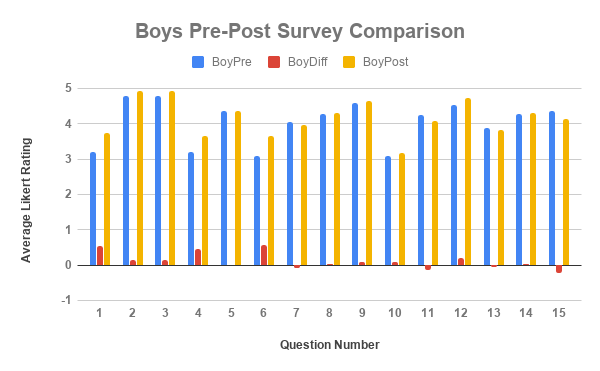
\includegraphics[width=3.3in]{images/boys}
\caption{Survey data: Boys}
\label{figure:boys}
\end{figure}

\begin{figure}
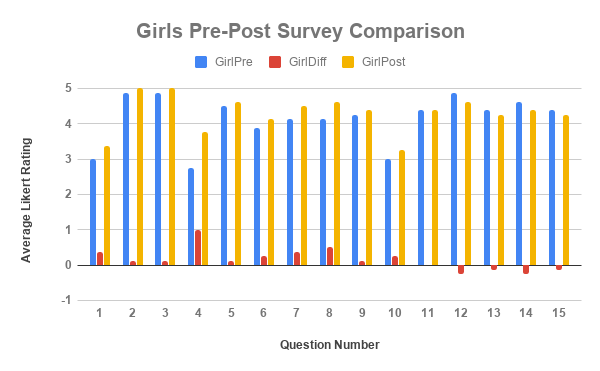
\includegraphics[width=3.3in]{images/girls}
\caption{Survey data: Girls}
\label{figure:girls}
\end{figure}

Figures \ref{figure:boys} and \ref{figure:girls} illustrate the changes
among both boys ($n=26$) and girls ($n=8$).
Informally, we saw an increase in student responses on all questions
except questions 11 (\textit{I want to learn more about computing}), 
13 (\textit{Solving problems is fun}), and 15 (\textit{I like computing}).
However, the decreases were not statistically significant at $\alpha\le 0.1$,
and the original rankings were relatively high (4.23, 3.88, and 4.35,
respectively).  Prior experience likely had some impact;
given that many had attended a prior camp, it was unclear whether this
new camp experience was likely to have an additional effect.

We ran a paired t-test using the pre-camp and post-camp surveys to
explore changes in students' attitudes.  In spite of camper prior
experience , we found statistically significant growth on questions
1 (\textit{I look like a computer scientist}, $p < 0.05$), 2
(\textit{Boys can do computing}, $p < 0.1$), 4 (\textit{I know a
lot about computing}, $p < 0.05$), and 6 (\textit{I know more than
my friends about computers}, $p < 0.05$).  We note that while there
was a statistically significant increase in the question 2 responses
and not in the question 3 responses, question 3 had a higher average
score on the pre-surveys and the average post-survey score for the two
questions was the same.

% Although we separately analyzed survey responses for boys and girls,
% we did not do a similar analysis for returners and new campers as
% the returning campers are a complicating factor.  For example, a
% new camper who masters material at a good rate may still consider
% themselves inferior to their peers who seem to know so much already.

\section{Discussion}

Because we had a comparatively small number of campers, surprisingly
few female participants (an issue we will discuss further), and a
large number of repeat participants, we do not feel confident
claiming that this curriculum has had a significant effect on the
students.  Nonetheless, it is worth exploring both the data and
some informal observations we made during the camp.

We were surprised at the initial responses to questions 2 (\textit{Boys
can do computing}) and 3 (\textit{Girls can do computing}).  We did
not expect either the high levels of agreement with those statements
or the similarities of responses from boys and girls, particularly
given that boys usually agree less about girls' ability to do
computing.  It may be that schools are doing a better job of
encouraging students to think broadly.  However, since these students
come from a variety of school districts, it may be that returning
students had already embraced this broader notion of who can do
computing.

We also admit that we were both surprised and frustrated by the
small number of female students enrolling in the camps.  Our other
camps on code crafts and on computing for social good tend to draw
a nearly even mix of boys and girls.  It may be that our hypothesis
that the Digital Humanities would attract young women was incorrect.
It may be that we failed to advertise the camp appropriately---while
we thought a title of ``Language and Code'' would highlight the
humanistic aspect, it may be that many potential students read it
as ``programming language''.  We will need to revisit this question
if we are to offer the camp again.

\concept{Informal observations}
We also observed some effects that we could not easily measure.

One returning student, who had been reluctant to work with others
or to ask for help in the previous camp, thrived in this camp.  He not
only approached the project with enthusiasm, but showed great
flair in his presentation.

Although our primary goal is to promote computing, we also expect
that the camps can promote college.  During one of the scavenger
hunts, one of the campers said ``I never thought about attending
college.  But this place is cool.  Do you think I could get in?''
We assured him that with hard work, he could.

A visiting K-12 teacher noted that they appreciated the ways that
some of the exercises helped students think more deeply about
language, particularly the Madlibs and language generation projects.
It could be that this is a natural way to incorporate more computing
in language courses not so much to teach computing, but to help
students gain a deeper understanding of language.

\concept{Projects}
We had hoped that students would evenly distribute among the various
approaches to projects, drawing upon one or more of the methods
from the mini projects: Hypertext stories, language generation, Madlibs, 
text analysis, and Web page manipulation.  However, the
majority decided to write ``choose your own adventure'' stories.

There were, of course, exceptions.  Two teams adapted the basic Madlibs 
model.  Two teams worked with counselors to build more advanced
projects that combined Madlibs with hypertext stories.\footnote{While
the students could modify existing programs, it was clear that they
had not developed the mastery necessary to build more sophisticated
programs.  Counselors therefore provided additional support.}
In one case, the initial Madlibs answers carried from page to page,
so that characters and other words would reappear.  In the other,
students asked questions on each page and accumulated data for a
final page.  Two teams explored issues of language generation,
creating more complex texts and, in one case, attempting to including
rhyming in poems.  
A few teams avoided the ``language and code'' theme.
One built a time-wasting click counter.  A second started
a role-playing-style fighting game with character stats.  A
third built a single page collection of useful links with affiliated
images.\footnote{Twenty years ago, they might have been as
innovative as Yahoo.}

In spite of these few detours, we consider the projects a success.
Students worked hard on their projects, posters, and presentations.
We also saw pride in their projects.  Many parents and campers
called and emailed after the camp asking for access to the projects.

\concept{Difficulties}
That is not to say that the camp was a complete success.  As we
have already noted, we are frustrated to have attracted such a small
fraction of female campers.  It is also clear that we threw too
much at the campers; by the time we got to the Web manipulation
exercises on day four, many seemed lost.  It appears that our
approach of ``focus more on concepts than underlying details'' may
not have been the best approach if we wanted students to branch
beyond the examples we provided.  While we have given the students
a sense of power, particularly in their ability to create Web pages
and hypertext stories that they can share on the Web, it may be
that we have given them too little power to think computationally.

\section{Conclusions and Future Work}

The underrepresentation of many groups in computing remains an issue
of national concern, not only because computing has the potential
to provide fulfilling and rewarding career opportunities, but also
because the nation needs people from a wide variety of perspectives
building the technology that so frequently affects our daily lives.
Although many approaches have started to make some difference, it
is clear the computer science education and computing communities
must continue to explore new ways to attract and support members
of underrepresented groups.  It's clear that no one method will
work; we need a spectrum of approaches to support a range of
people and perspectives.

In this paper, we have explored one particular approach, the use
of language-based computing exercises associated with the Digital
Humanities in a code camp for middle-school students.  Our experience
in this project was mixed.  While students enjoyed the camp
and we saw a few changes in attitude, the camp failed to attract a
large number of students from our target groups.  And we clearly
packed too much material into a one-week camp.

Unfortunately, the size and character of the camper population made
it difficult to show success or failure of the curriculum.  Because
we had so many returning students, we do not know what the effects
on confidence or interest would have been on a cohort consisting
of only students who had not attended a previous camp.

We may not offer this camp a second time.  It is clear that if we
do, we will need to make a variety of changes, cutting back on the
number of activities and finding ways to better encourage a broader
variety of projects.  We will also need to find new ways to show
the applicability of the topic.

Nonetheless, we do see a role for exercises drawn from DH as a tool
in broadening participation in computing.  As noted, the language
generation and Madlibs exercises can help student learn not only
about computing, but also about language.  It may be that the
projects are better used individually, in the context of other
outreach activities, rather than combined into a single week-long
experience.  We also consider it worth exploring uses of DH
at the college level as an avenue to broadening participation.

For those interested in adapting any of our work, the curriculum,
slide decks, instructors guides, and worksheets are available online
at https://codecamp.sites.grinnell.edu/languageandcode/.
